\documentclass{article}

\usepackage{tikz_imports}

\begin{document}

\newcommand{\AxisRotator}[1][rotate=0] {%
  \tikz[decoration={
    markings,
    mark=at position 1 with {\arrow{latex}}}]\draw[x = .5em, y = 2.75em, line width = .2ex,#1,postaction=decorate] (0,0)  arc (-150:150:.45 and .5) -- ++(-95:2pt);%                                                   
  }


\begin{figure}[ht]
\centering

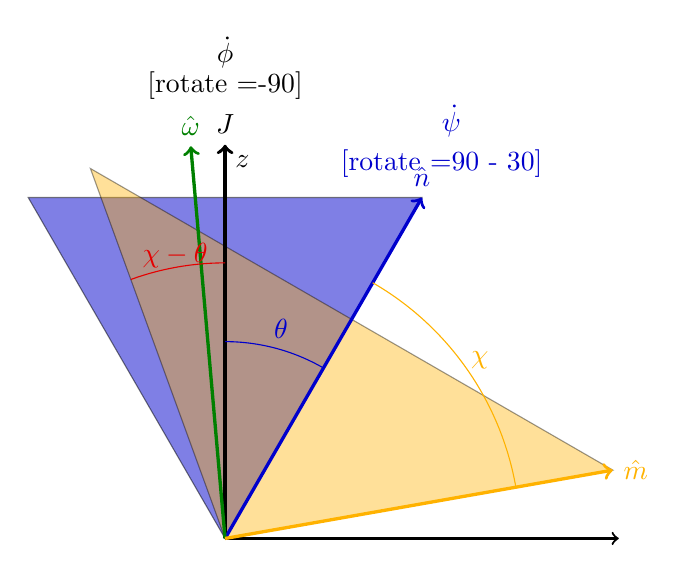
\begin{tikzpicture}[scale=5]

%define angles
\pgfmathsetmacro{\thetaang}{30}
\pgfmathsetmacro{\chiang}{50}
\pgfmathsetmacro{\thetaanghat}{-5}

% Define some colors
\definecolor{deformation}{rgb}{0.0, 0, 0.8}
\definecolor{dipole}{rgb}{1.0, 0.7, 0.0}

% draw cones
\draw[fill = deformation, opacity=0.5] 
            (0, 0)  -- ({sin(\thetaang)}, {cos(\thetaang)}) --   
           % ({sin(\thetaang)}, {cos(\thetaang)}) arc (90 - \thetaang: 90+\thetaang :1) --
            ({sin(-\thetaang)}, {cos(-\thetaang)}) --cycle;

\draw[fill = dipole, opacity=0.4] 
            (0, 0)  -- ({sin(\thetaang + \chiang)}, {cos(\thetaang + \chiang)}) --  
           %({sin(\thetaang + \chiang)}, {cos( \thetaang + \chiang)}) arc (90 - (\thetaang + \chiang) : 90-(\thetaang - \chiang)  :1) --
            ({sin(\thetaang - \chiang)}, {cos(\thetaang - \chiang)}) --cycle;

%draw the main coordinate system axes
\draw[thick,->] (0,0) -- (1,0) node[anchor=north east]{$$};
\draw[thick,->] (0,0) -- (0,1) node[anchor = north west]{$z$};



%draw lines
\draw[very thick, black, ->] (0,0) -- (0, 1.0) node[above]{$\boldsymbol{J}$};
\draw[very thick, deformation,, ->] (0,0) -- ({sin(\thetaang)}, {cos(\thetaang)}) node[above]{$\hat{\boldsymbol{n}}$};
\draw[very thick, green!50!black, ->] (0,0) -- ({sin(\thetaanghat)}, {cos(\thetaanghat)}) node[above]{$\hat{\boldsymbol{\omega}}$};
\draw[very thick, dipole, ->] (0,0) --  ({sin(\thetaang + \chiang)}, {cos(\thetaang + \chiang)}) node[anchor=west]{$\hat{\boldsymbol{m}}$};


% draw angle arcs
\draw[deformation] ({0.5 * sin(\thetaang)}, {0.5 * cos(\thetaang)})  arc (90 - \thetaang: 90: 0.5);
\node[deformation] at ({0.55 * sin(0.5 * \thetaang)}, { 0.55 * cos(0.5 * \thetaang)}){$\theta$} ;

\draw[dipole] ({0.75 * sin(\chiang + \thetaang)}, {0.75 * cos(\chiang + \thetaang)})  arc (90 - (\thetaang + \chiang): 90 - \thetaang: 0.75);
\node[dipole] at ({0.79 * sin(0.5 * \chiang + \thetaang)}, { 0.79 * cos(0.5 * \chiang + \thetaang)}){$\chi$} ;

%\draw[purple] (0, 0.6)  arc (90: 116-(2*\thetaang - \chiang): 0.75);
%\node[purple] at ({-0.79 * cos(2*\chiang-\thetaang)},{0.79 * sin(2*\chiang-\thetaang)}){$2\theta - \chi$} ;

% Draw rotation
\draw[color=black] (0.0,0.0) node at (0.,1.15) {\AxisRotator[rotate =-90]} ;
\node[above] at (0, 1.17) {$\dot{\phi}$};

\draw[color=deformation] (0.0,0.0) node at ({1.1*sin(\thetaang)}, {1.1*cos(\thetaang)}) {\AxisRotator[rotate =90 - \thetaang]} ;
\node[above,  color=deformation] at ({1.15*sin(\thetaang)}, {1.15*cos(\thetaang)}) {$\dot{\psi}$};


\draw[red!90!black] (0, 0.7)  arc (90: 90-(\thetaang - \chiang): 0.7);
\node[red!90!black] at ({-0.73 * sin(.5*(\chiang-\thetaang))},{0.73 * cos(.5*(\chiang-\thetaang))}){$\chi- \theta$} ;

\end{tikzpicture}
\end{figure}
\end{document}